\subsection{Half-Wave Rectifier With Filter:}

Using basically the same circuit of the Figure 3.2.0, we are going to connect in parallel to the {\bfseries\itshape $R_{L}$ resistor} a {\bfseries\itshape electrolytic capacitor}, this device will act like a filter. The voltage coming out from rectifiers is not smooth and a filter rectifier circuit is used to smoothen it for more stable constant DC voltage. We are going to be exchanging between two different capacitors, one of $470\mu F$ and another of $2200\mu F$.

\begin{figure}[H]
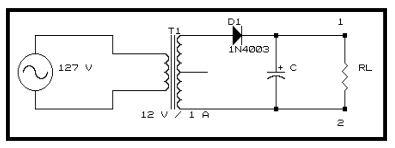
\includegraphics[scale=.8]{rhalf-wave.png}
\centering \linebreak \linebreak Figure 3.3.0: Half-wave rectifier circuit with filter.
\end{figure} 

Once the circuit it's armed using the $100\Omega\ resistor\ as\ R_{L}$ we will measure with the voltmeter the {\bfseries\itshape Voltage} and {\bfseries\itshape Current} in this component. According to the Figure 3.3.0, we will connect the Positive terminal of the voltmeter in the terminal 1 of Figure 3.3.0 and the Negative terminal of the voltmeter in the terminal 2 of Figure 3.3.0, we will call this voltage $V_{0}$ for the current $I_{0}$ we can use {\bfseries\itshape Ohm's Law}: \hfill \break

{\bfseries\itshape\color{Maroon}{Using Ohm's Law: $I_{0} = \frac{V_{0}}{R_{L}}.$}} \hfill \break

\begin{center}
\begin{tabular}[.5cm]{l c c c}
\toprule
Capacitor & $V_{0}$ & $I_{0}$ \\
\midrule
470$\mu F$ & 14.6 $V$ & 0.146 A \\
\cmidrule{1-3}
2200$\mu F$ & 15.06 $V$ & 0.150 A \\
\bottomrule
\linebreak
\end{tabular}
\centering \linebreak Table 2: Measured values of Figure 3.3.0.
\end{center} \hfill

The small unwanted residual periodic variation of the direct current (DC) output of a power supply which has been derived from an alternating current (AC) source it's called {\bfseries\itshape Ripple}. To measure the {\bfseries\itshape ripple voltage $\Delta$V} it's necessary to connect the {\bfseries\itshape oscilloscope terminals} in the terminals 1 and 2 of the Figure 3.3.0 in the option of AC.

\begin{multicols}{2}
\begin{itemize}
\item Using the 470$\mu F$ capacitor:
\end{itemize}

\begin{figure}[H]
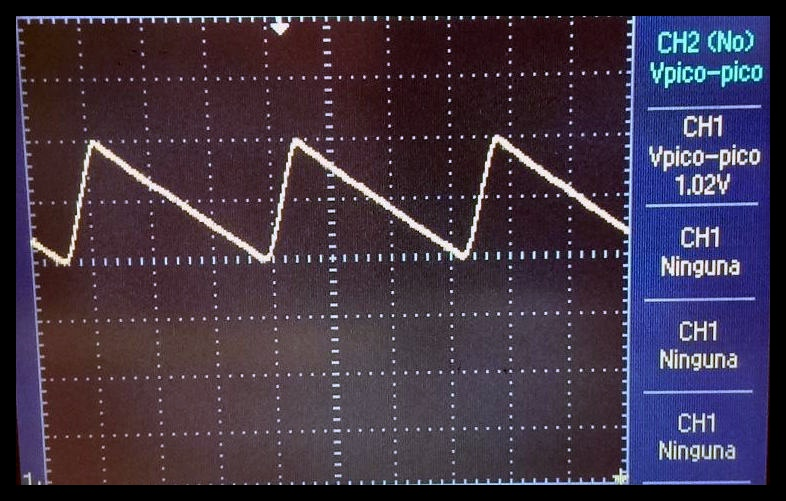
\includegraphics[scale=.3]{o1.jpg}
\centering \linebreak \linebreak Figure 3.3.1: Half-wave with filter rectified signal.
\linebreak .\linebreak $\frac{2 V}{div}\ \ and\ \ \frac{5mseg}{div}$.
\end{figure}

\begin{itemize}
\item Using the 2200$\mu F$ capacitor:
\end{itemize}

\begin{figure}[H]
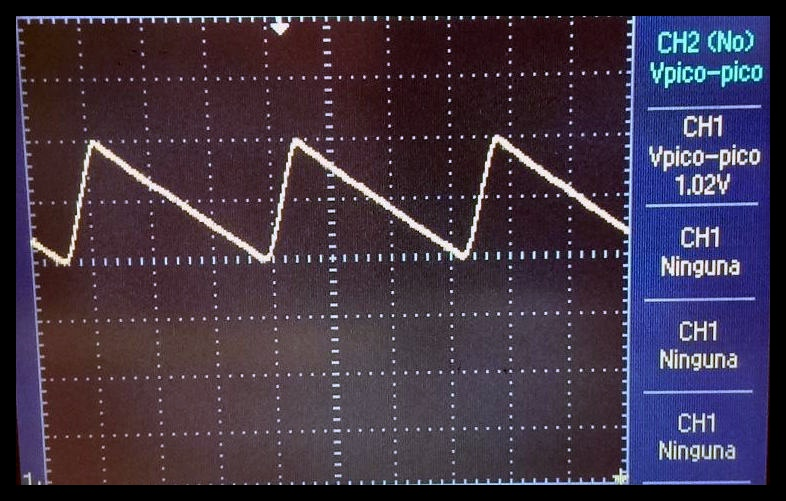
\includegraphics[scale=.3]{o1.jpg}
\centering \linebreak \linebreak Figure 3.3.2: Half-wave with filter rectified signal.
\linebreak \linebreak $\frac{500 mV}{div}\ \ and\ \ \frac{5mseg}{div}$.
\end{figure}
\end{multicols}

{\bfseries\itshape
\begin{itemize}
\item For the ripple voltage ( $\Delta$V ):
\end{itemize}}

When the terminals of the oscilloscope are connected to the circuit and the signal it's displayed on screen as Figures 3.3.1 and 3.3.2 shows. We will put the oscilloscope in the option of {\bfseries\itshape measures} and the {\bfseries\itshape ripple} voltage will be the {\bfseries\itshape peak-to-peak voltage ( $V_{pp}$ )}. \hfill \break

\begin{center}
\begin{tabular}[.5cm]{l c c }
\toprule
Capacitor & $\Delta V$  \\
\midrule
470$\mu F$ & 4.48 $V$ \\
\cmidrule{1-2}
2200$\mu F$ & 1.02 $V$ \\
\bottomrule
\linebreak
\end{tabular}
\centering \linebreak Table 3: Ripple Voltage of Figure 3.3.0.
\end{center} \hfill

\pagebreak